\documentclass[landscape,12pt]{amsart}
\usepackage[pdftex]{graphicx}
\usepackage{tikz}
\usepackage{hyperref}

\setlength{\paperwidth}{1189mm}
\setlength{\paperheight}{841mm}
\setlength{\topmargin}{10mm}
\setlength{\oddsidemargin}{10mm}
\setlength{\evensidemargin}{10mm}
\setlength{\headheight}{0mm}
\setlength{\headsep}{0mm}
\setlength{\topskip}{0mm}
\setlength{\footskip}{0mm}
\setlength{\textwidth}{1169mm}
\setlength{\textheight}{821mm}
%\special{papersize=84.1cm,59.4cm}
%\setpapersize{A1}

\newcommand{\xx}{190mm}
\newcommand{\yy}{330mm}
\newcommand{\ww}{250mm}
\newcommand{\vv}{35mm}

\newcommand{\R}{\mathbb{R}}
\newcommand{\Z}{\mathbb{Z}}
\newcommand{\tm}{\times}
\newcommand{\tht}{\theta}
\newcommand{\Smash}{\wedge}
\newcommand{\spec}{\operatorname{spec}}
\newcommand{\Hom}{\operatorname{Hom}}
\newcommand{\OO}{\mathcal{O}}
\newcommand{\st}{\;|\;}
\newcommand{\sse}{\subseteq}
\newcommand{\psb}[1]{[\![#1]\!]}
\newcommand{\pp}{\hphantom{-}}
\newcommand{\mm}{-}
\newcommand{\tai}{\tau^{-1}}
\newcommand{\bbm}       {\left[\begin{matrix}}
\newcommand{\ebm}       {\end{matrix}\right]}
\newcommand{\blob}      {circle(0.03cm)}

\DeclareMathOperator{\Tet}      {Tet}
\DeclareMathOperator{\Cube}     {Cube}
\DeclareMathOperator{\Oct}      {Oct}
\DeclareMathOperator{\Dodec}    {Dodec}
\DeclareMathOperator{\Icos}     {Icos}

\DeclareMathOperator{\Aut}      {Aut}
\DeclareMathOperator{\Dir}      {Dir}
\DeclareMathOperator{\Fix}      {Fix}
\DeclareMathOperator{\Trans}    {Trans}
\DeclareMathOperator{\Isom}     {Isom}
\DeclareMathOperator{\Symm}     {Symm}



\renewcommand{\:}{\colon}

\renewcommand{\section}[1]{\begin{center}\Huge #1\end{center}\vspace{10mm}}
\newenvironment{pg}{%
\begin{minipage}[t][\yy][t]{\xx}\par\vspace*{10mm}%
}{%
\end{minipage}
}

\begin{document}%
\fontfamily{phv}\selectfont
\pagestyle{empty}

\includegraphics[scale=0.4]{logo}%
\hspace{220mm}\raisebox{20mm}{\fontsize{100}{100}\selectfont 
Symmetries of Platonic solids}\\
\vspace{30mm}
\noindent
\framebox[\ww]{\begin{pg}
\section{The Platonic solids}

\begin{center}
 \begin{tikzpicture}[scale=1.4]
  \draw ( 0.0, 3.0) node {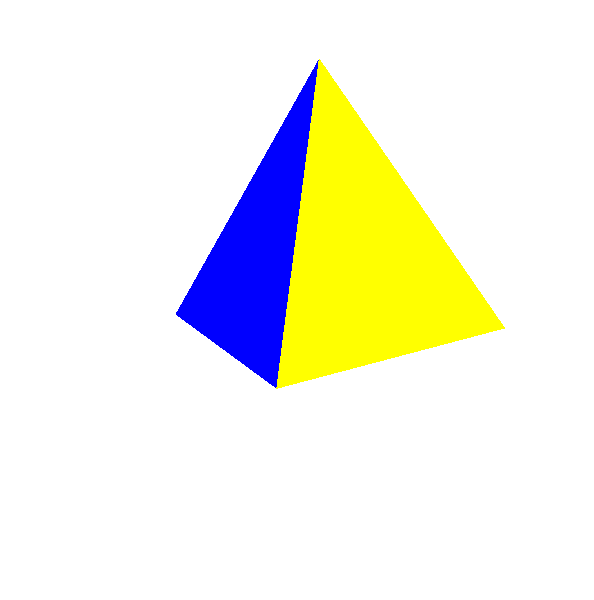
\includegraphics[scale=0.7]{pdf/tetra}};
  \draw (-4.0, 0.0) node {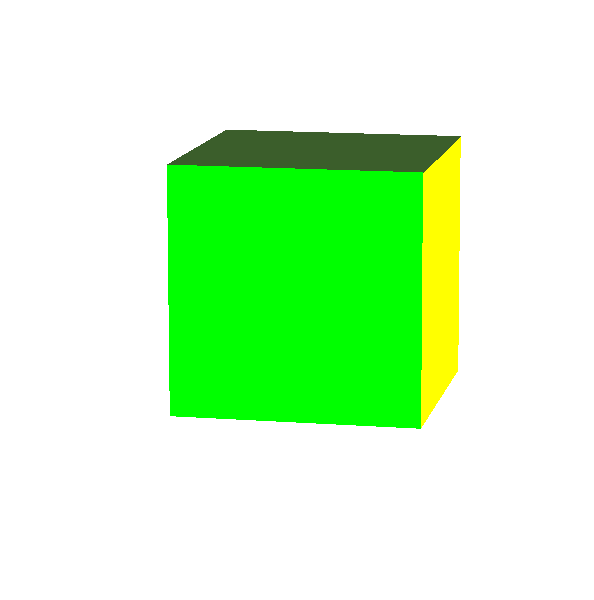
\includegraphics[scale=0.7]{pdf/cube}};
  \draw ( 4.0, 0.0) node {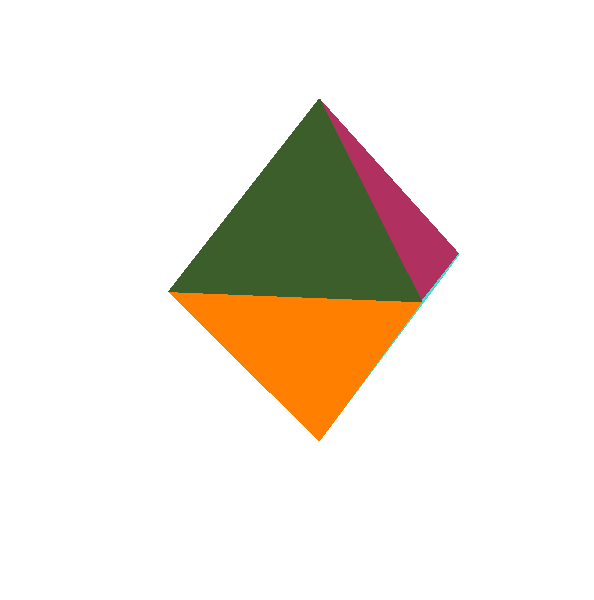
\includegraphics[scale=0.8]{pdf/oct}};
  \draw ( 3.0,-4.0) node {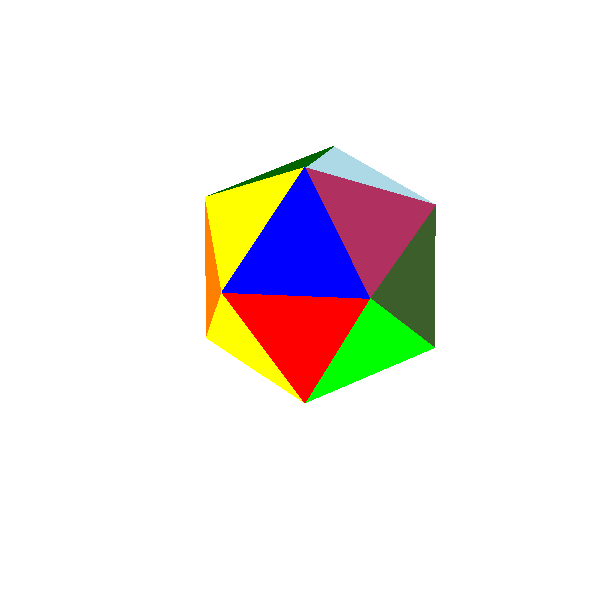
\includegraphics[scale=0.9]{pdf/icos}};
  \draw (-3.0,-4.0) node {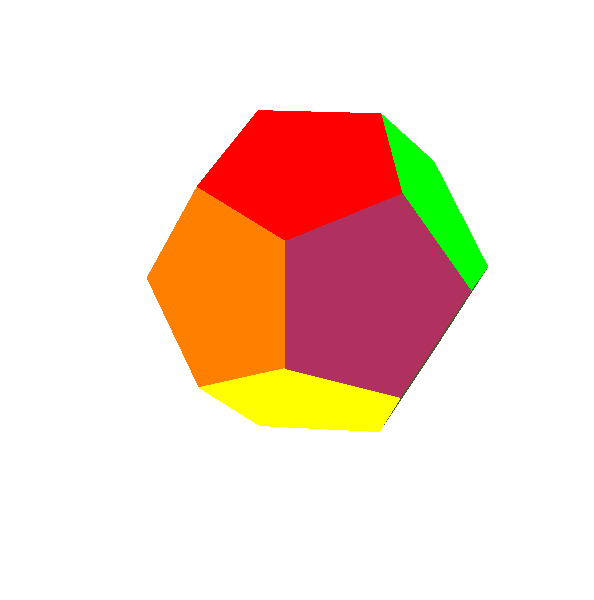
\includegraphics[scale=0.7]{pdf/dodec}};
 \end{tikzpicture}
\end{center}

 \bigskip

 The five Platonic solids are the tetrahedron, cube, octahedron,
 dodecahedron and icosahedron.  \\ They are related to the finite
 subgroups of the rotation group 
 \[ SO(3) = \{A\in M_3(\R)\st A^TA=I,\; \det(A)=1\} \]
 and the slightly larger group 
 \[ O(3) = \{A\in M_3(\R)\st A^TA=I\} = SO(3)\tm\{\pm I\}. \]

 If $X$ is a Platonic solid centred at the origin, then the sets 
 \[ \Dir(X) = \{A\in O(3)\st AX=X\} \qquad\text{ and } \qquad
    \Symm(X) = \Dir(X)\cap SO(3)
 \]
 are nontrivial finite subgroups of $O(3)$ and $SO(3)$.  It can be
 shown that any finite subgroup of $SO(3)$ is either cyclic or
 dihedral or conjugate to $\Symm(X)$ for some Platonic solid $X$.

\end{pg}}\hspace{\vv}%
%%%%%%%%%%%%%%%%%%%%%%%%%%%%%%%%%%%%%%%%%%%%%%%%%%%%%%%%%%%%%%%%%%%%%%
\framebox[\ww]{\begin{pg}%
\section{The Tetrahedron}

The tetrahedron has 4 vertices, 6 edges and 4 faces, each of which is
an equilateral triangle.  There are 6 planes of reflectional symmetry,
one of which is shown on the below.  Each such plane contains one edge
and bisects the opposite edge (this gives one plane for each edge,
hence 6 planes).  Reflection in a plane fixes two of the vertices and
exchanges the other two, so the corresponding vertex permutation is a
transposition.
\[ 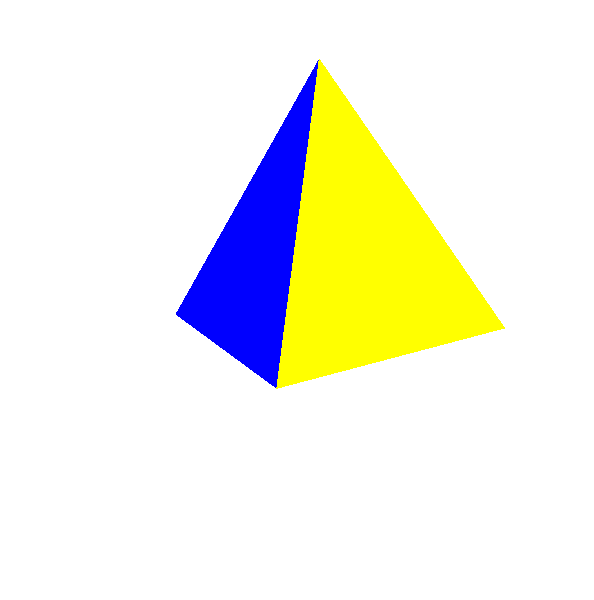
\includegraphics[scale=0.8]{pdf/tetra} 
   \hspace{3em}
   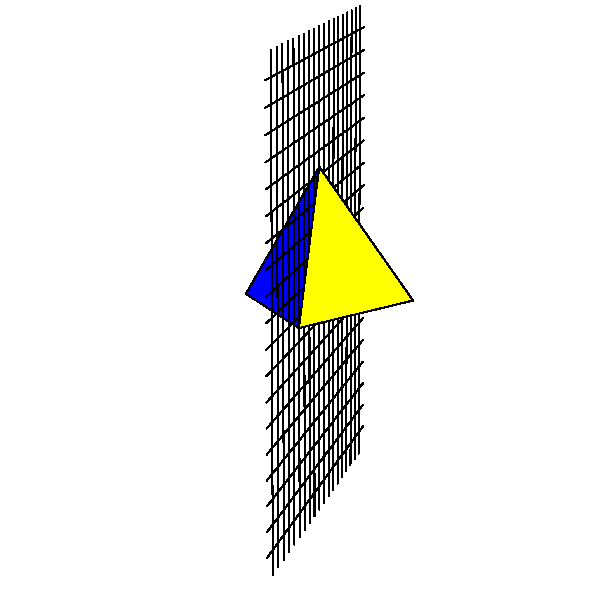
\includegraphics[scale=0.8]{pdf/tetraref} 
\]
There are 4 lines of 3-fold rotational symmetry, each of which passes
through a vertex and the centre of the opposite face (giving one line
for each vertex).  These are shown below in red.  The corresponding
vertex permutations are 3-cycles.

There are also 3 lines of 2-fold rotational symmetry, shown in green.
Each one joins the centres of an opposite pair of edges.  The
corresponding edge permutations are transposition pairs, in other
words they have the form $(a b)(c d)$ where $a$, $b$, $c$
and $d$ are all different. 
\[ 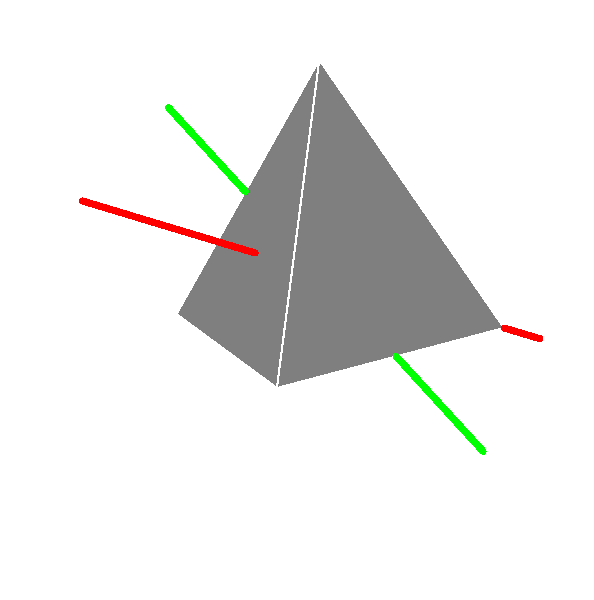
\includegraphics[scale=0.8]{pdf/tetrarot} 
   \hspace{3em}
   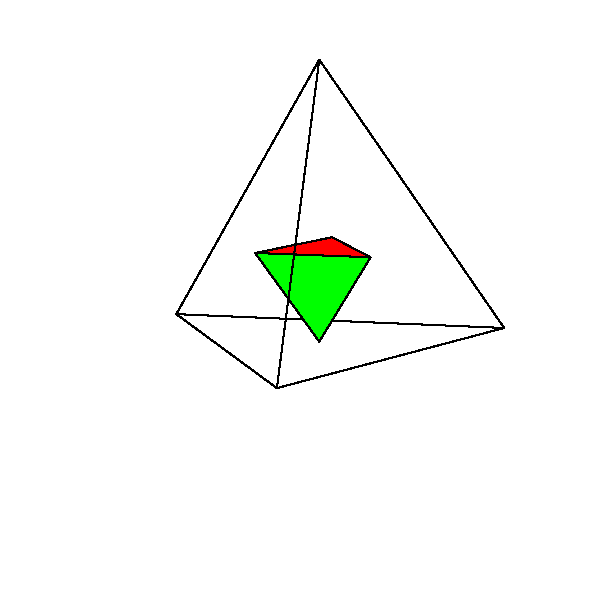
\includegraphics[scale=0.8]{pdf/tetradual} 
\]
If we start with a tetrahedron (such as the wire frame above) and find
the centres of all the faces we get the vertices of a new tetrahedron
(the coloured one).  Thus, the tetrahedron is self-dual.



\end{pg}}\hspace{\vv}%
%%%%%%%%%%%%%%%%%%%%%%%%%%%%%%%%%%%%%%%%%%%%%%%%%%%%%%%%%%%%%%%%%%%%%%
\framebox[\ww]{\begin{pg}%
\section{The Cube}

The cube has 8 vertices, 12 edges and 6 faces, each of which is
a square.  There are rotational symmetries of order 2 (about the green
axis), order 3 (the red axis) and order 4 (the blue axis).
\[ 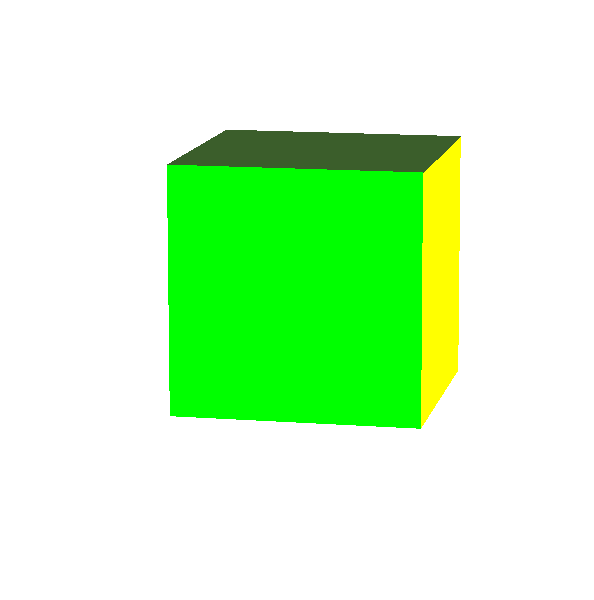
\includegraphics[scale=0.8]{pdf/cube} 
   \hspace{3em}
   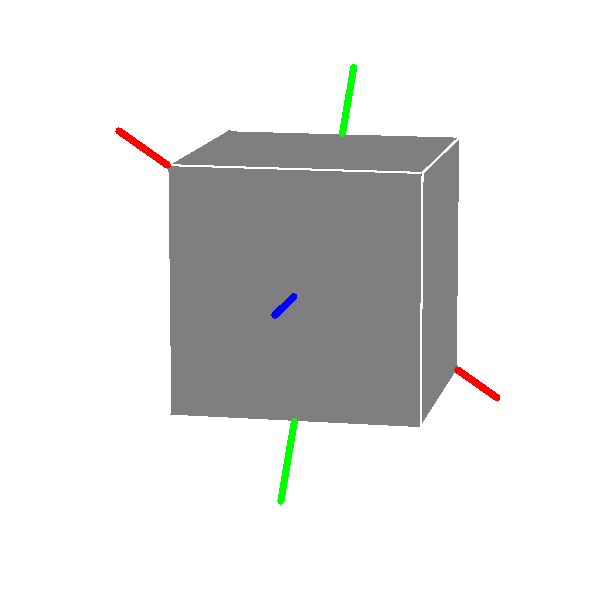
\includegraphics[scale=0.8]{pdf/cuberot} 
\]
The cube is also invariant under multiplication by -1, so
\[ \Dir(\Cube) = \Symm(\Cube) \tm \{1,-1\}. \]
There are 4 long diagonals (shown below), which are permuted by the
action of the symmetry group, giving rise to a homomorphism
\[ \phi\:\Symm(\Cube) \to S_4 \]
The rotations of orders 2, 3 and 4 are sent to 2-cycles,
3-cycles and 4-cycles respectively. It turns out that
$\phi$ is an isomorphism.
\[ 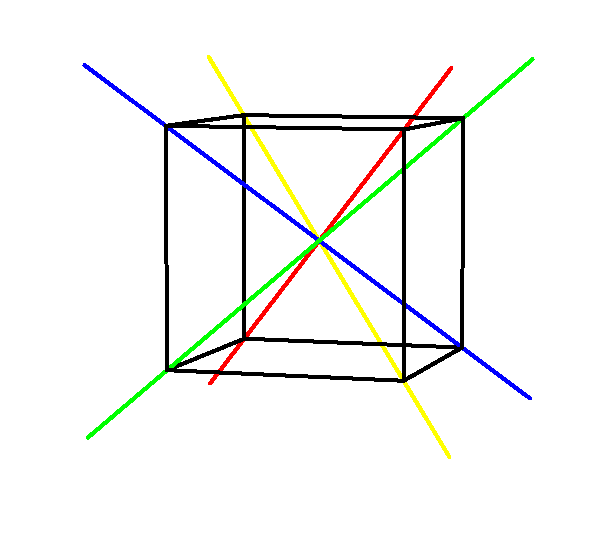
\includegraphics[scale=0.8]{pdf/cubediag} 
   \hspace{3em}
   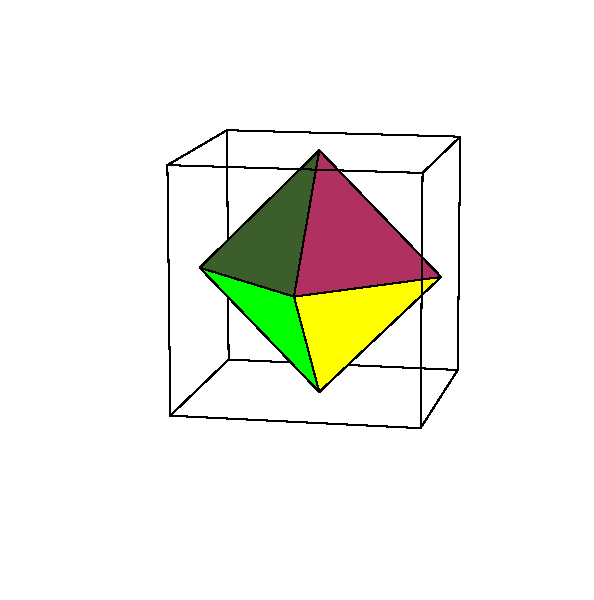
\includegraphics[scale=0.8]{pdf/cubedual} 
\]
If we start with a cube (such as the wire frame above) and find
the centres of all the faces we get the vertices of an octahedron.  In
other words, the dual of a cube is an octahedron.

\bigskip

The vertices of the cube are 
\begin{align*}
 a_0 &= (\pp 1,\pp 1,\pp 1) & 
 a_1 &= (\pp 1,\pp 1,\mm 1) & 
 a_2 &= (\pp 1,\mm 1,\pp 1) & 
 a_3 &= (\pp 1,\mm 1,\mm 1) \\
 a_4 &= (\mm 1,\pp 1,\pp 1) & 
 a_5 &= (\mm 1,\pp 1,\mm 1) & 
 a_6 &= (\mm 1,\mm 1,\pp 1) & 
 a_7 &= (\mm 1,\mm 1,\mm 1),
\end{align*}
and the faces are 
\begin{align*}
 B_0 &: \pp x=1 & B_1 &: \pp y=1 & B_2 &: \pp z = 1 \\
 B_3 &: \mm x=1 & B_4 &: \mm y=1 & B_5 &: \mm z = 1.
\end{align*}

\end{pg}}\hspace{\vv}%
%%%%%%%%%%%%%%%%%%%%%%%%%%%%%%%%%%%%%%%%%%%%%%%%%%%%%%%%%%%%%%%%%%%%%%
\framebox[\ww]{\begin{pg}%
\section{The Octahedron}

The octahedron has 6 vertices, 12 edges and 8 faces, each of which is
an equilateral triangle.  There are rotational symmetries of order 2 
(about the green axis), order 3 (the red axis) and order 4 (the blue axis).
\[ 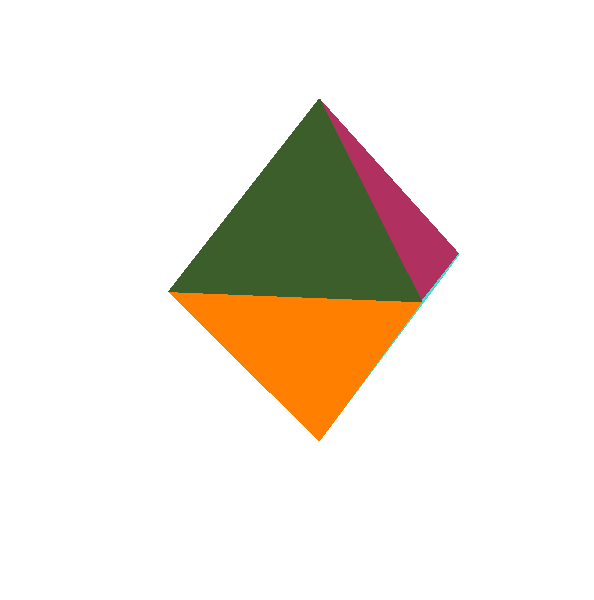
\includegraphics[scale=0.8]{pdf/oct} 
   \hspace{3em}
   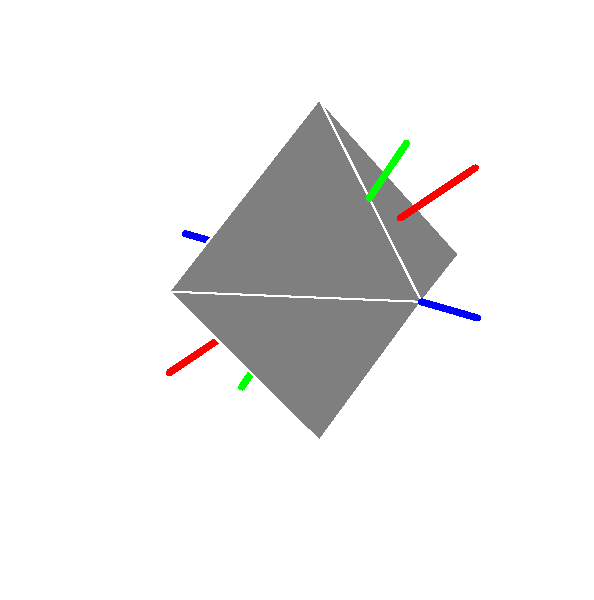
\includegraphics[scale=0.8]{pdf/octrot} 
\]
The dual of an octahedron is a cube:
\[ 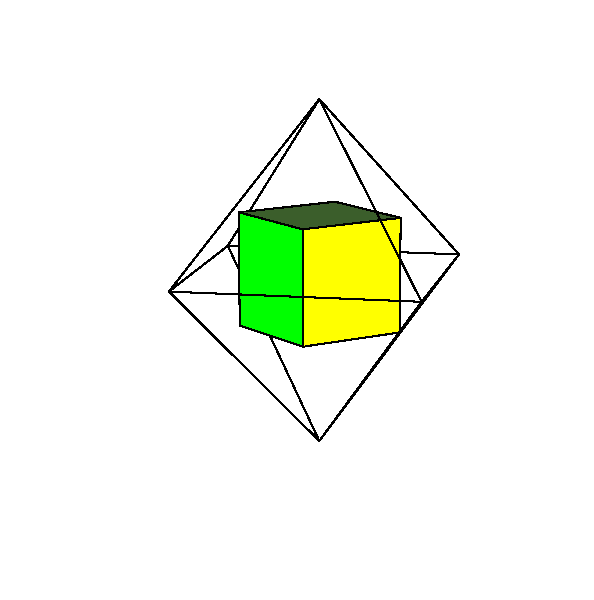
\includegraphics[scale=1.2,trim=0cm 1cm 0cm 1cm,clip]{pdf/octdual} \]
As dual polyhedra have the same symmetry groups, we have
\[ \Symm(\Oct) = \Symm(\Cube) = S_4. \]

\bigskip
The vertices of the octahedron are 
\begin{align*}
 b_0 &= (\pp 1,\pp 0,\pp 0) & 
 b_1 &= (\pp 0,\pp 1,\pp 0) & 
 b_2 &= (\pp 0,\pp 0,\pp 1) \\ 
 b_3 &= (\pp 1,\pp 0,\pp 0) & 
 b_4 &= (\pp 0,\mm 1,\pp 0) & 
 b_5 &= (\pp 0,\pp 0,\mm 1),
\end{align*}
and the faces are
\begin{align*}
 A_0 &: \pp x  +  y  +  z = 1 & 
 A_1 &: \pp x  +  y \mm z = 1 & 
 A_2 &: \pp x \mm y  +  z = 1 & 
 A_3 &: \pp x \mm y \mm z = 1 \\
 A_4 &: \mm x  +  y  +  z = 1 & 
 A_5 &: \mm x  +  y \mm z = 1 & 
 A_6 &: \mm x \mm y  +  z = 1 & 
 A_7 &: \mm x \mm y \mm z = 1. 
\end{align*}

The algebraic manifestation of duality is that the equation of $A_i$
is $(x,y,z).a_i=1$, and the equation of $B_j$ is $(x,y,z).b_j=1$.

\end{pg}}\\[15mm]
%%%%%%%%%%%%%%%%%%%%%%%%%%%%%%%%%%%%%%%%%%%%%%%%%%%%%%%%%%%%%%%%%%%%%%
\framebox[\ww]{\begin{pg}%
\section{The Dodecahedron}

The dodecahedron has 20 vertices, 30 edges and 12 faces,
each of which is a regular pentagon.  There are rotational symmetries
of order $2$ (around the blue axis), order $3$ (around the green axis)
and order $5$ (around the red axis).
\[ 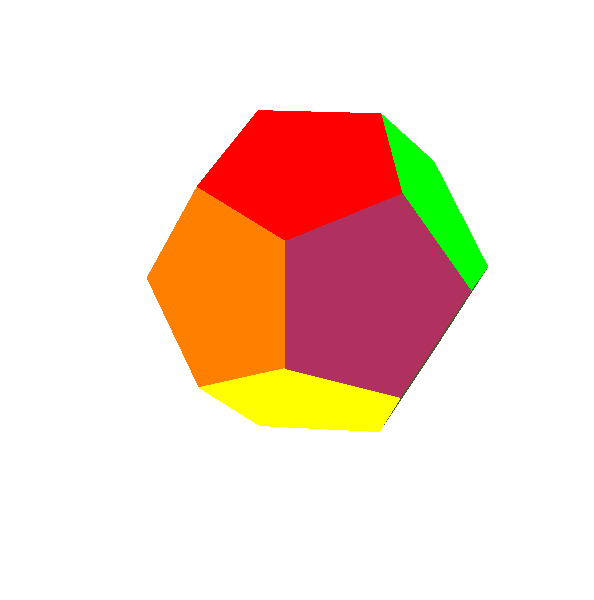
\includegraphics[scale=0.8]{pdf/dodec} 
   \hspace{3em}
   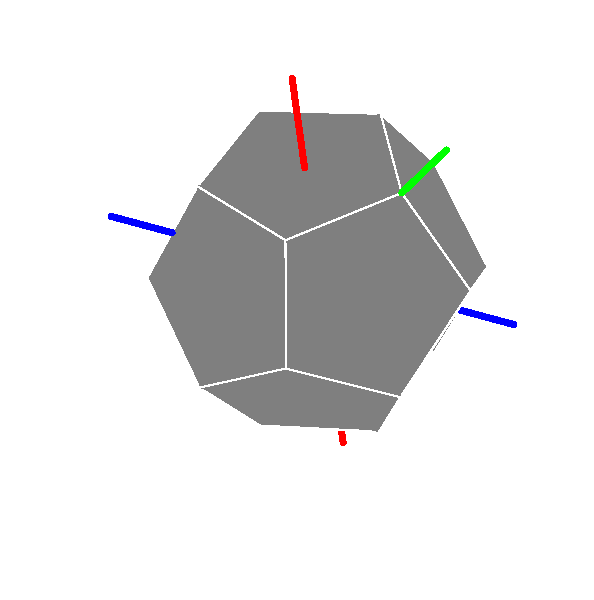
\includegraphics[scale=0.8]{pdf/dodecrot} 
\]
By joining each vertex to the opposite one, we obtain 10 different
lines of 3-fold rotational symmetry.  We can twist around each of
these axes by an angle of $2\pi/3$ or $4\pi/3$, giving 20 different
rotations of order 3.  By joining the centre of each face to the
centre of the opposite face, we obtain 6 different lines of 5-fold
rotational symmetry, giving 24 rotations of order 5.  By joining the
centre of each edge to the centre of the opposite edge, we obtain 15
different lines of 2-fold rotational symmetry.

The vertices are the vertices $a_0,\dotsc,a_7$ of the cube, together
with twelve more.  We can write the coordinates in terms of the
``golden ratio'' $\tau=(\sqrt{5}+1)/2$ and its inverse
$\tau^{-1}=(\sqrt{5}-1)/2$: 

\begin{align*}
 a_{ 8} &= (0,\pp\tai,\pp\tau) &
 a_{ 9} &= (\pp\tau,0,\pp\tai) &
 a_{10} &= (\pp\tai,\pp\tau,0) \\
 a_{11} &= (0,\pp\tai,\mm\tau) &
 a_{12} &= (\mm\tau,0,\pp\tai) &
 a_{13} &= (\pp\tai,\mm\tau,0) \\
 a_{14} &= (0,\mm\tai,\pp\tau) &
 a_{15} &= (\pp\tau,0,\mm\tai) &
 a_{16} &= (\mm\tai,\pp\tau,0) \\
 a_{17} &= (0,\mm\tai,\mm\tau) &
 a_{18} &= (\mm\tau,0,\mm\tai) &
 a_{19} &= (\mm\tai,\mm\tau,0).
\end{align*}

In each of these vectors, one entry is zero, one is $\pm\tau$ and one
is $\pm\tai$.  The following picture shows how the cube fits inside
the dodecahedron:
\[ 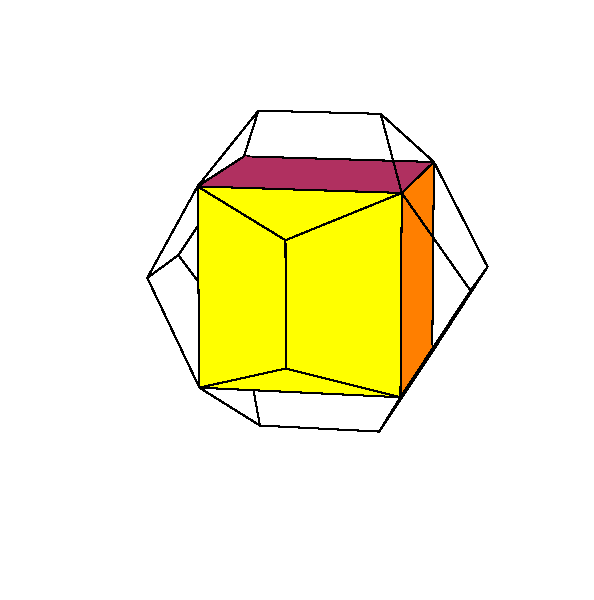
\includegraphics[scale=1.0]{pdf/incube} \]


\end{pg}}\hspace{\vv}%
%%%%%%%%%%%%%%%%%%%%%%%%%%%%%%%%%%%%%%%%%%%%%%%%%%%%%%%%%%%%%%%%%%%%%%
\framebox[\ww]{\begin{pg}%

 Some detailed analysis is needed to show that the faces fit together
 neatly.

 \vspace{3ex}

 \begin{center}
  \begin{tikzpicture}[scale=4] % [60]{-2}{2}{-1.7}{2.3}
   \draw (0.592,-0.384) -- (-2.21,-0.103) -- (-0.866,1.07) -- (0.866,0.898) --
          (0.592,-0.384) -- (2.21,0.103) -- (0.866,0.898);
   \draw[dashed] (2.21,0.103) -- (-0.592,0.384) -- (-0.866,1.07);
   \draw[dashed] (-0.592,0.384) -- (-2.21,-0.103);
   \draw[dotted] (0.809,0.243) -- (-0.809,-0.243);
   \draw[dotted] (1.4,-0.14) -- (-1.4,0.14);
   \draw ( 2.35, 0.123) node {$\scriptstyle{A}$};
   \draw (-0.80, 0.469) node {$\scriptstyle{B}$};
   \draw ( 0.60,-0.480) node {$\scriptstyle{C}$};
   \draw (-2.35,-0.123) node {$\scriptstyle{D}$};
   \draw (-0.95, 1.190) node {$\scriptstyle{E}$};
   \draw ( 0.95, 1.000) node {$\scriptstyle{F}$};
   \draw[very thick] (0,0) -- (0,0.985) -- (-0.809,-0.243) -- (0,0);
   \draw (-0.135,0.55) node {$\scriptstyle{\alpha}$};
   \draw[very thick] (1.4,-0.14) -- (0.866,-0.0868) -- (0.866,0.898) -- (1.4,-0.14);
   \draw (1.17,0.0305) node {$\scriptstyle{\beta}$};
  \end{tikzpicture}
 \end{center}

 \vspace{10ex}

 \begin{center}
  \begin{tikzpicture}[scale=3] % [60]{-2}{1}{-0.5}{1.5}
   \draw[very thick] (0,0) -- (-1.6,0) -- (0,1) -- (0,0);
   \draw (-1.7,0) node[anchor=east]
    {${\textstyle\frac{1}{2}}(C+D)$};
   \draw (0.1,1) node[anchor=west]
    {${\textstyle\frac{1}{2}}(E+F)$};
   \draw (-0.8,-0.1) node[anchor=north] {$1/2$};
   \draw (0.1,0.5) node[anchor=west] {$1/(2\tau)$};
   \draw (-0.1,0.8) node {$\alpha$};
  \end{tikzpicture} 
  \hspace{3em}
  \begin{tikzpicture}[scale=3] % [60]{-1}{2}{-0.5}{1.5}
   \draw[very thick] (0,0) -- (0.6,0) -- (0,1) -- (0,0);
   \draw (-0.1,1) node[anchor=east] {$F$};
   \draw (0.7,0) node[anchor=west] {${\tfrac{1}{2}}(A+C)$};
   \draw (0.3,-0.1) node[anchor=north] {$(1-\tau^{-1})/2$};
   \draw (-0.1,0.5) node[anchor=east] {$1/(2\tau)$};
   \draw (0.4,0.1) node {$\beta$};
  \end{tikzpicture} 
 \end{center}

 \vspace{10ex}

 \begin{center}
  \begin{tikzpicture}[scale=2.4] % [50]{-1.3}{1.8}{-1.2}{1.5}
   \draw (0.296,-0.989) -- (1.11,-0.745) -- (1.38,-0.0385) -- (0.884,-0.189) --
          (0.296,-0.989) -- (0.296,0.605) -- (0.884,-0.189) -- (1.38,-0.0385) --
          (1.11,0.848) -- (0.433,1.25) -- (0.296,0.605) -- (-1.11,0.745) --
          (-0.433,1.33) -- (0.433,1.25) -- (1.11,0.848);
   \draw (0.296,-0.989) -- (-1.11,-0.848) -- (-1.11,0.745);
   \draw[dashed] (1.11,-0.745) -- (1.11,0.848) -- (-0.296,0.989) --
                 (-0.296,-0.605) -- (1.11,-0.745);
   \draw[dashed] (-1.11,0.745) -- (-0.296,0.989) -- (-0.433,1.33);
   \draw[dashed] (-1.11,-0.848) -- (-0.296,-0.605);
   \fill (0.433,1.25) \blob;
   \fill (0.296,0.605) \blob;
   \fill (0.884,-0.189) \blob;
   \draw (0.44,1.35) node[anchor=south west] {$P$};
   \draw (0.28,0.50) node[anchor=north east] {$Q$};
   \draw (0.8,-0.19) node[anchor=east] {$R$};
   \draw[very thick] (0.296,0.605) -- (1.11,0.848);
  \end{tikzpicture}
  \hspace{5em}
  \begin{tikzpicture}[scale=1.5] % [25]{-3}{3}{-2}{2.9}
   \draw (-1.6,-1.6) -- (1.6,-1.6) -- (1.6,1.6) -- (-1.6,1.6) -- (-1.6,-1.6) --
          (-1.6,1.6) -- (-1,2.6) -- (1,2.6) -- (1.6,1.6) -- (2.6,0) -- (1.6,-1.6);
   \draw[dotted] (-1.8,0) -- (2.8,0);
   \fill (1.0,2.6) \blob;
   \fill (1.6,1.6) \blob;
   \fill (2.6,0.0) \blob;
   \draw (1.1,2.7) node[anchor=south west] {$P$};
   \draw (1.7,1.7) node[anchor=south west] {$Q$};
   \draw (2.7,0.1) node[anchor=south west] {$R$};
   \draw (2.3,0.2) node {$\alpha$};
   \draw (1.3,1.8) node {$\beta$};
  \end{tikzpicture} 
 \end{center}
\end{pg}}\hspace{\vv}%
%%%%%%%%%%%%%%%%%%%%%%%%%%%%%%%%%%%%%%%%%%%%%%%%%%%%%%%%%%%%%%%%%%%%%%
\framebox[\ww]{\begin{pg}%

We can actually inscribe 5 different cubes in a dodecahedron; they
are shown in 5 different colours below.  Note that each face
contains exactly one line of each colour.

\[ 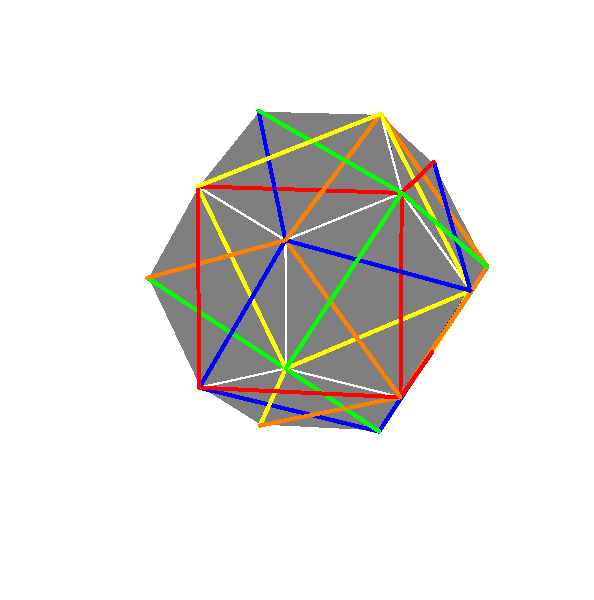
\includegraphics[scale=1]{pdf/incubes} \]

The symmetry group acts on the set of inscribed cubes, giving a
homomorphism 
\[ \phi\:\Symm(\Dodec) \to S_5 \] 

Some explicit rotation matrices in $\Symm(\Dodec)$ are given below:
\[ 
 R_2 = \bbm 1 & 0 & 0 \\ 0 & -1 & 0 \\ 0 & 0 & -1 \ebm 
 \hspace{3em}
 R_3 = \bbm 0 & 1 & 0 \\ 0 & 0 & 1 \\ 1 & 0 & 0 \ebm 
 \hspace{3em}
 R_5 = \frac{1}{2}
   \bbm \tai & -1 & \tau \\ 1 & \tau & \tai \\ -\tau & \tai & 1 \ebm.
\]
One can check that $\phi(R_5)$ is a $5$-cycle, $\phi(R_3)$ is a
$3$-cycle and $\phi(R_2)$ is a product of two disjoint transpositions.
It can be shown using this that $\phi$ is actually an isomorphism
$\Symm(\Dodec)\to A_5$.

\bigskip

The dual of a dodecahedron is an icosahedron.
\[ 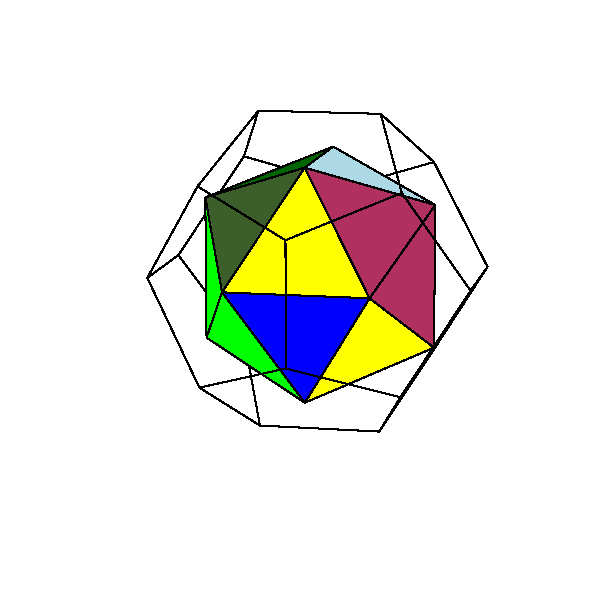
\includegraphics[scale=1.0]{pdf/dodecdual} \]


\end{pg}}\hspace{\vv}%
%%%%%%%%%%%%%%%%%%%%%%%%%%%%%%%%%%%%%%%%%%%%%%%%%%%%%%%%%%%%%%%%%%%%%%
\framebox[\ww]{\begin{pg}%

\section{The Icosahedron}

The icosahedron has 12 vertices, 30 edges and 20 faces, each of which
is an equilateral triangle.  There are rotational symmetries
of order $2$ (around the blue axis), order $3$ (around the green axis)
and order $5$ (around the red axis).
\[ 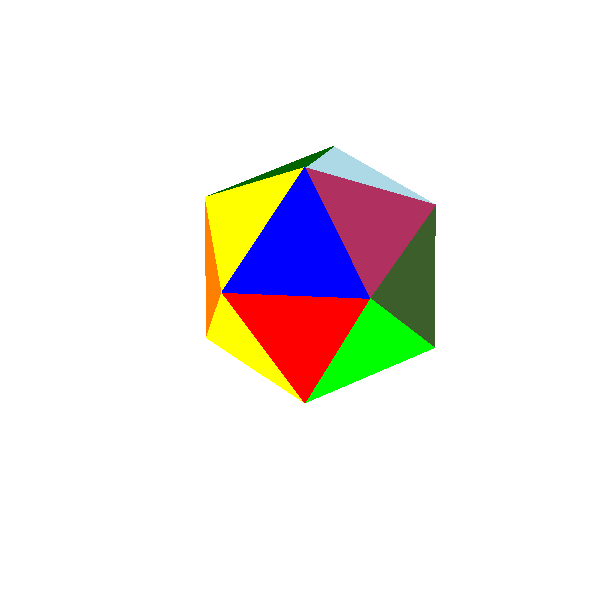
\includegraphics[scale=1.0]{pdf/icos} 
   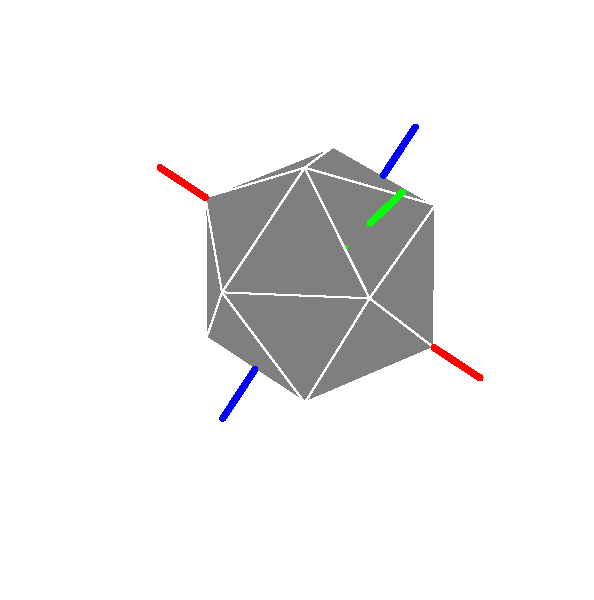
\includegraphics[scale=1.0]{pdf/icosrot} 
\]
The icosahedron is dual to the dodecahedron and so has the same
symmetry group.
\[ 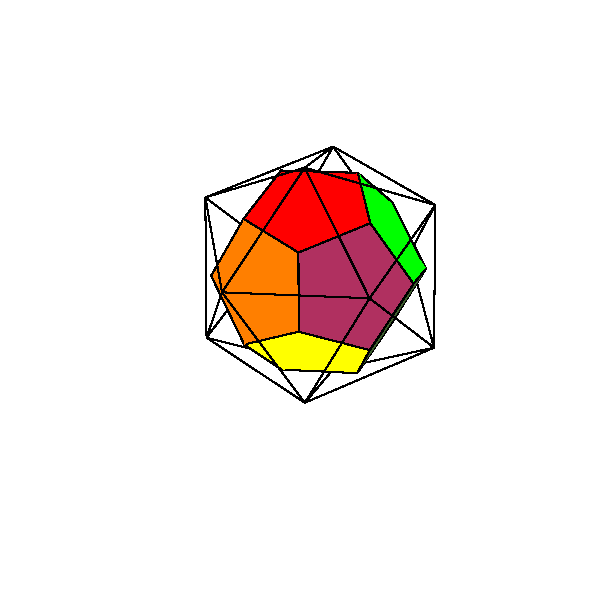
\includegraphics[scale=1.2,trim=0cm 3cm 0cm 2cm,clip]{pdf/icosdual} \]
This is also the same as the symmetry group of a football or the
Buckminsterfullerene molecule.
\[ 
\includegraphics[scale=0.10]{pdf/football}
   \hspace{5em} 
   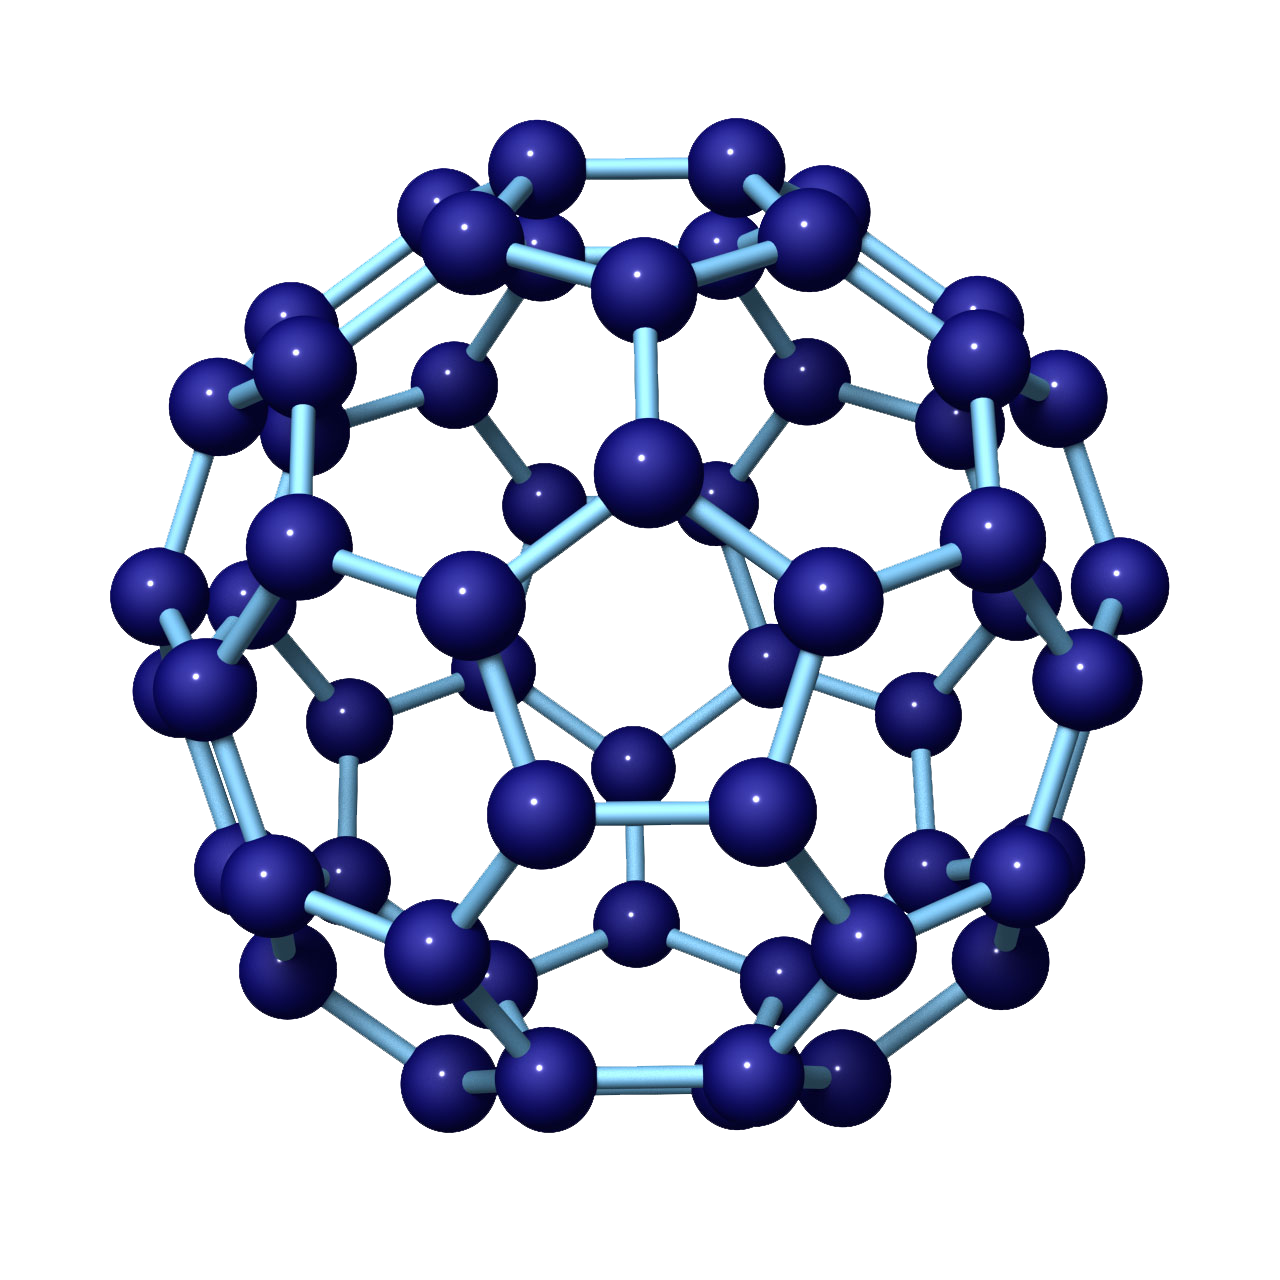
\includegraphics[scale=0.12,trim=0cm 2cm 0cm 0cm,clip]{pdf/buckyball} 
\]

\end{pg}}%
\\[20mm]
Poster by Neil Strickland
\end{document}
%%%%%%%%%%%%%%%%%%%%%%%%%%%%%%%%%%%%%%%%%%%%%%%%%%%%%%%%%%%%%%%%%%%%%%
%%%%%%%%%%%%%%%%%%%%%%%%%%%%%%%%%%%%%%%%%%%%%%%%%%%%%%%%%%%%%%%%%%%%%%
%%%%%%%%%%%%%%%%%%%%%%%%%%%%%%%%%%%%%%%%%%%%%%%%%%%%%%%%%%%%%%%%%%%%%%
%%%%%%%%%%%%%%%%%%%%%%%%%%%%%%%%%%%%%%%%%%%%%%%%%%%%%%%%%%%%%%%%%%%%%%
%%%%%%%%%%%%%%%%%%%%%%%%%%%%%%%%%%%%%%%%%%%%%%%%%%%%%%%%%%%%%%%%%%%%%%







\end{document}
